\documentclass[a4paper, 12pt, ngerman]{article}

% ======================================================================
% Packages
% ======================================================================
\usepackage{babel}
\usepackage[utf8]{inputenc}
\usepackage[T1]{fontenc}
\usepackage{CormorantGaramond}
\usepackage[scaled = 0.92]{helvet}
\usepackage{geometry}
\usepackage{fancyhdr}
\usepackage{tikz}
\usetikzlibrary{shapes}
\usetikzlibrary{arrows}
\usetikzlibrary{decorations}
\usetikzlibrary{decorations.markings}
\usetikzlibrary{calc}
\usetikzlibrary{intersections}
\usepackage{eurosym}
\usepackage{hyperref}
% ======================================================================

\def\kaiserName{Mikhail Pak}
\def\kaiserEmail{mikhail.pak@tum.de}
\def\headerLeft{%
  \resizebox{!}{1 cm}{%
    
\begin{tikzpicture}
      \node[inner sep = 0 pt, outer sep = 0 pt, text width = 10 cm, align = left] %
        at (0, 0) {%
          \fontfamily{phv}\selectfont\color{tum blue}%
          Lehrstuhl für Regelungstechnik\\
          Fakultät für Maschinenwesen\\
          Technische Universität München
        };
    \end{tikzpicture}
  }
}
\def\headerRight{%
  \resizebox{!}{1 cm}{%
    
\begin{tikzpicture}
      \path[fill=tum blue]
        (0.1649, 0.8021) -- (0.0000, 0.8021) --
        (0.0000, 1.0000) -- (0.7347, 1.0000) --
        (0.7347, 0.2028) -- (0.9109, 0.2028) --
        (0.9109, 1.0000) -- (1.8716, 1.0000) --
        (1.8716, 0.0000) -- (1.6653, 0.0000) --
        (1.6653, 0.7930) -- (1.4884, 0.7930) --
        (1.4884, 0.0000) -- (1.2842, 0.0000) --
        (1.2842, 0.7930) -- (1.1098, 0.7930) --
        (1.1098, 0.0000) -- (0.5326, 0.0000) --
        (0.5326, 0.8021) -- (0.3642, 0.8021) --
        (0.3642, 0.0000) -- (0.1663, 0.0000) --
        cycle;
    \end{tikzpicture}
  }
}

% ======================================================================
% TUM-Farben
% ======================================================================
\definecolor{tum blue}{HTML}{0065BD}
\definecolor{tum green}{HTML}{A2AD00}
\definecolor{tum orange}{HTML}{E37222}
\definecolor{tum ivory}{HTML}{DAD7CB}

\definecolor{tum dia violet}{HTML}{69085A}
\definecolor{tum dia dark blue}{HTML}{0F1B5F}
\definecolor{tum dia turquoise}{HTML}{00778A}
\definecolor{tum dia dark green}{HTML}{007C30}
\definecolor{tum dia light green}{HTML}{679A1D}
\definecolor{tum dia light yellow}{HTML}{FFDC00}
\definecolor{tum dia dark yellow}{HTML}{F9BA00}
\definecolor{tum dia dark orange}{HTML}{D64C13}
\definecolor{tum dia red}{HTML}{C4071B}
\definecolor{tum dia dark red}{HTML}{9C0D16}
% ======================================================================


% ======================================================================
% Einrückungen und Zeilenabstand
% ======================================================================
\setlength\parindent{0pt}
\setlength\parskip{2 pt plus 1 pt minus 1 pt}
% ======================================================================


% ======================================================================
% Seitenlayout
% ======================================================================
\geometry{
  head     = 1.2 cm,
  headsep  = 1.4 cm,
  top      = 4.5 cm,
  right    = 2.4 cm,
  left     = 2.4 cm,
  foot     = 1.0 cm,
  footskip = 2.0 cm,
  bottom   = 3.0 cm,
}
% ======================================================================


% ======================================================================
% Kopf- und Fußzeilen
% ======================================================================
\pagestyle{fancy}

% Keine Linien
\renewcommand{\headrulewidth}{0pt}
\renewcommand{\footrulewidth}{0pt}

\fancyhead[L]{\headerLeft}
\fancyhead[C]{}
\fancyhead[R]{\headerRight}

\fancyfoot[L]{}
\fancyfoot[C]{}
\fancyfoot[R]{}
% ======================================================================


% ======================================================================
% hyperref
% ======================================================================
\hypersetup{
    pdffitwindow    = false,
    pdfstartview    = FitH,
    pdftitle        = {},
    pdfauthor       = {},
    pdfkeywords     = {},
    pdfnewwindow    = false,
    colorlinks      = false,
    linkcolor       = black,
    urlcolor        = black,
    citecolor       = black,
    allbordercolors = black!10,
    urlcolor        = black,
}
% ======================================================================



\begin{document}

\fontfamily{phv}\selectfont

\begin{verbatim}
                                     .
                                      `:.
                                        `:.
                                .:'     ,::
                               .:'      ;:'
                               ::      ;:'
                                :    .:'
                                 `.  :.
                        _________________________
                       : _ _ _ _ _ _ _ _ _ _ _ _ :
                   ,---:".".".".".".".".".".".".":
                  : ,'"`::.:.:.:.:.:.:.:.:.:.:.::'
                  `.`.  `:-===-===-===-===-===-:'
                    `.`-._:                   :
                      `-.__`.               ,' met.
                  ,--------`"`-------------'--------.
                   `"--.__                   __.--"'
                          `""-------------""'
\end{verbatim}

\vspace*{5 mm}

\begin{center}
  \LARGE \textbf{Preis pro Tasse (alle Sorten): \EUR{0,25}}
\end{center}

\large

\begin{itemize}
  \item[--] Bitte halten Sie die Küche sauber!


  \item[--] Tragen Sie für jede Tasse Kaffee ein Kreuz in die Liste ein,
  von oben nach unten und von links nach rechts (siehe Bild):
  \begin{center}
    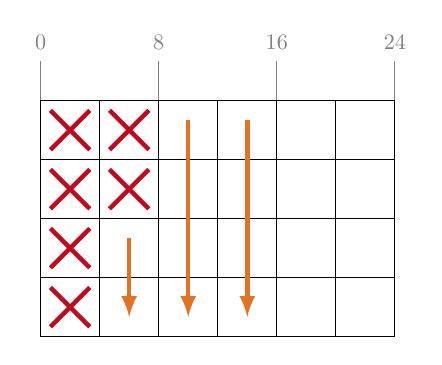
\begin{tikzpicture}[scale = 2.5]
      \foreach \i in {0, 1, ..., 4} {\draw (4.2, -0.6 + \i*0.3) -- +(1.8, 0);}
      \foreach \i in {0, 1, ..., 6} {\draw (4.2 + \i*0.3, -0.6) -- +(0, 1.2);}

      \draw[ultra thick, tum dia red] (4.2 + 0.15, 0.45) %
        +(0.1, 0.1) -- +(-0.1, -0.1) %
        +(-0.1, 0.1) -- +(0.1, -0.1);
      \draw[ultra thick, tum dia red] (4.2 + 0.15, 0.15) %
        +(0.1, 0.1) -- +(-0.1, -0.1) %
        +(-0.1, 0.1) -- +(0.1, -0.1);
      \draw[ultra thick, tum dia red] (4.2 + 0.15, -0.15) %
        +(0.1, 0.1) -- +(-0.1, -0.1) %
        +(-0.1, 0.1) -- +(0.1, -0.1);
      \draw[ultra thick, tum dia red] (4.2 + 0.15, -0.45) %
        +(0.1, 0.1) -- +(-0.1, -0.1) %
        +(-0.1, 0.1) -- +(0.1, -0.1);
      \draw[ultra thick, tum dia red] (4.2 + 0.45, 0.45) %
        +(0.1, 0.1) -- +(-0.1, -0.1) %
        +(-0.1, 0.1) -- +(0.1, -0.1);
      \draw[ultra thick, tum dia red] (4.2 + 0.45, 0.15) %
        +(0.1, 0.1) -- +(-0.1, -0.1) %
        +(-0.1, 0.1) -- +(0.1, -0.1);

      \draw[ultra thick, tum orange, -latex] (4.2 + 0.45, -0.1) -- +(0, -0.4);
      \draw[ultra thick, tum orange, -latex] (4.2 + 0.75, 0.5) -- +(0, -1);
      \draw[ultra thick, tum orange, -latex] (4.2 + 1.05, 0.5) -- +(0, -1);

      \foreach \i in {0, 8, ..., 24} {
        \draw[black!50] (4.2 + \i*0.075, 0.6) -- +(0, 0.2) %
        node[outer sep = 2 pt, scale = 0.8, above] {\i};
      }
    \end{tikzpicture}
  \end{center}


  \item[--] Bei Fragen wenden Sie sich an \kaiserName (\url{\kaiserEmail}).
\end{itemize}

\vfill

\footnotesize Bildquelle: \url{http://ascii.co.uk/art/cup}.

\end{document}
